% Quelqu'un a pensé à faire une intro ??

\chapter{Mesures d'admittances sur instruments à corde pincée}
\vspace{5mm}
\paragraph*{Objectifs}

Dans le but de fournir aux deux systèmes de synthèse l'admittance d'instruments
à cordes (guitare, ukulélé...), nous devons en faire la mesure sur les
instruments réels. Pour cela il est nécessaire 

\begin{itemize}
\item[$\bullet$] d'identifier des grandeurs physiques utile pour les synthèses
\item[$\bullet$] de mettre en place un dispositif de mesures d'admittance
\item[$\bullet$] d'établir un protocole de mesures avec système d'acquisition 
\item[$\bullet$] de visualiser et d'exploiter ces résultats 
\end{itemize}

%\paragraph*{Application : guitare}

\paragraph*{Nomenclature de la séance de mesure : \\} 
\begin{itemize}
\item $Y_{\text{corps},indice}$ : Admittance du corps. l'indice $1$ indique l'axe vertical et l'indice $2$ l'axe horizontal.
\item $Y_{\text{corde},indice}$ : Admittance de la corde.
\item $Y_{\text{total},note,indice}$ : Admittance de l'ensemble corde+corps.
\item $F$ : Force appliquée par le marteau 
\item $\alpha$ : Accélération délivrée par le capteur 
\end{itemize}

\subsection*{Identification des grandeurs pour les synthèses}

Pour la synthèse FRF et la synthèse modale nous avons besoin du
$Y_{\text{corps}}$ ainsi que du $Y_{\text{corde}}$ de la guitare. Nous pouvons
récupérer cette admittance dans deux dimensions grâce à un accéléromètre
multi-axe. La vibration de l'ensemble corde-corps de guitare est donnée par un
marteau d'impact, excitant le système au niveau du point de couplage (pour la
guitare, le chevalet). Nous récupèrerons également grâce à un microphone de
mesure la pression acoustique rayonnée à 2 mètres de la guitare. La synthèse
sonore pourra ainsi prendre en compte le rayonnement de la structure, ce qui
tend à donner plus de réalisme.

\subsection*{Dispositif de mesures}

Pour nos mesures, nous disposons d'un capteur, d'un marteau d'impulsion, d'une
carte d'acquisition NI, d'un amplificateur, d'un système d'acquisition sur
matlab, d'un microphone et enfin d'une guitare et d'un ukulele \\

Le capteur est un acceléromètre tri-axes, calibré dont on implémente la
sensibilité dans le code d'acquisition. Le marteau d'impulsion fourni la force
d'impacte $F$ sur la guitare. \\ Lors de l'acquisition de nos résultats, le
signal d'impulsion est fenétré pour enlever tout bruit électronique. \\ Au
final nous récupérons, la réponse temporelle de l'accélération en 2D et de la
force. On obtient également leur réponse fréquentielle, c'est le rapport des
deux, qui donne l'iadmittance du système.

\begin{figure}[h]
\centering
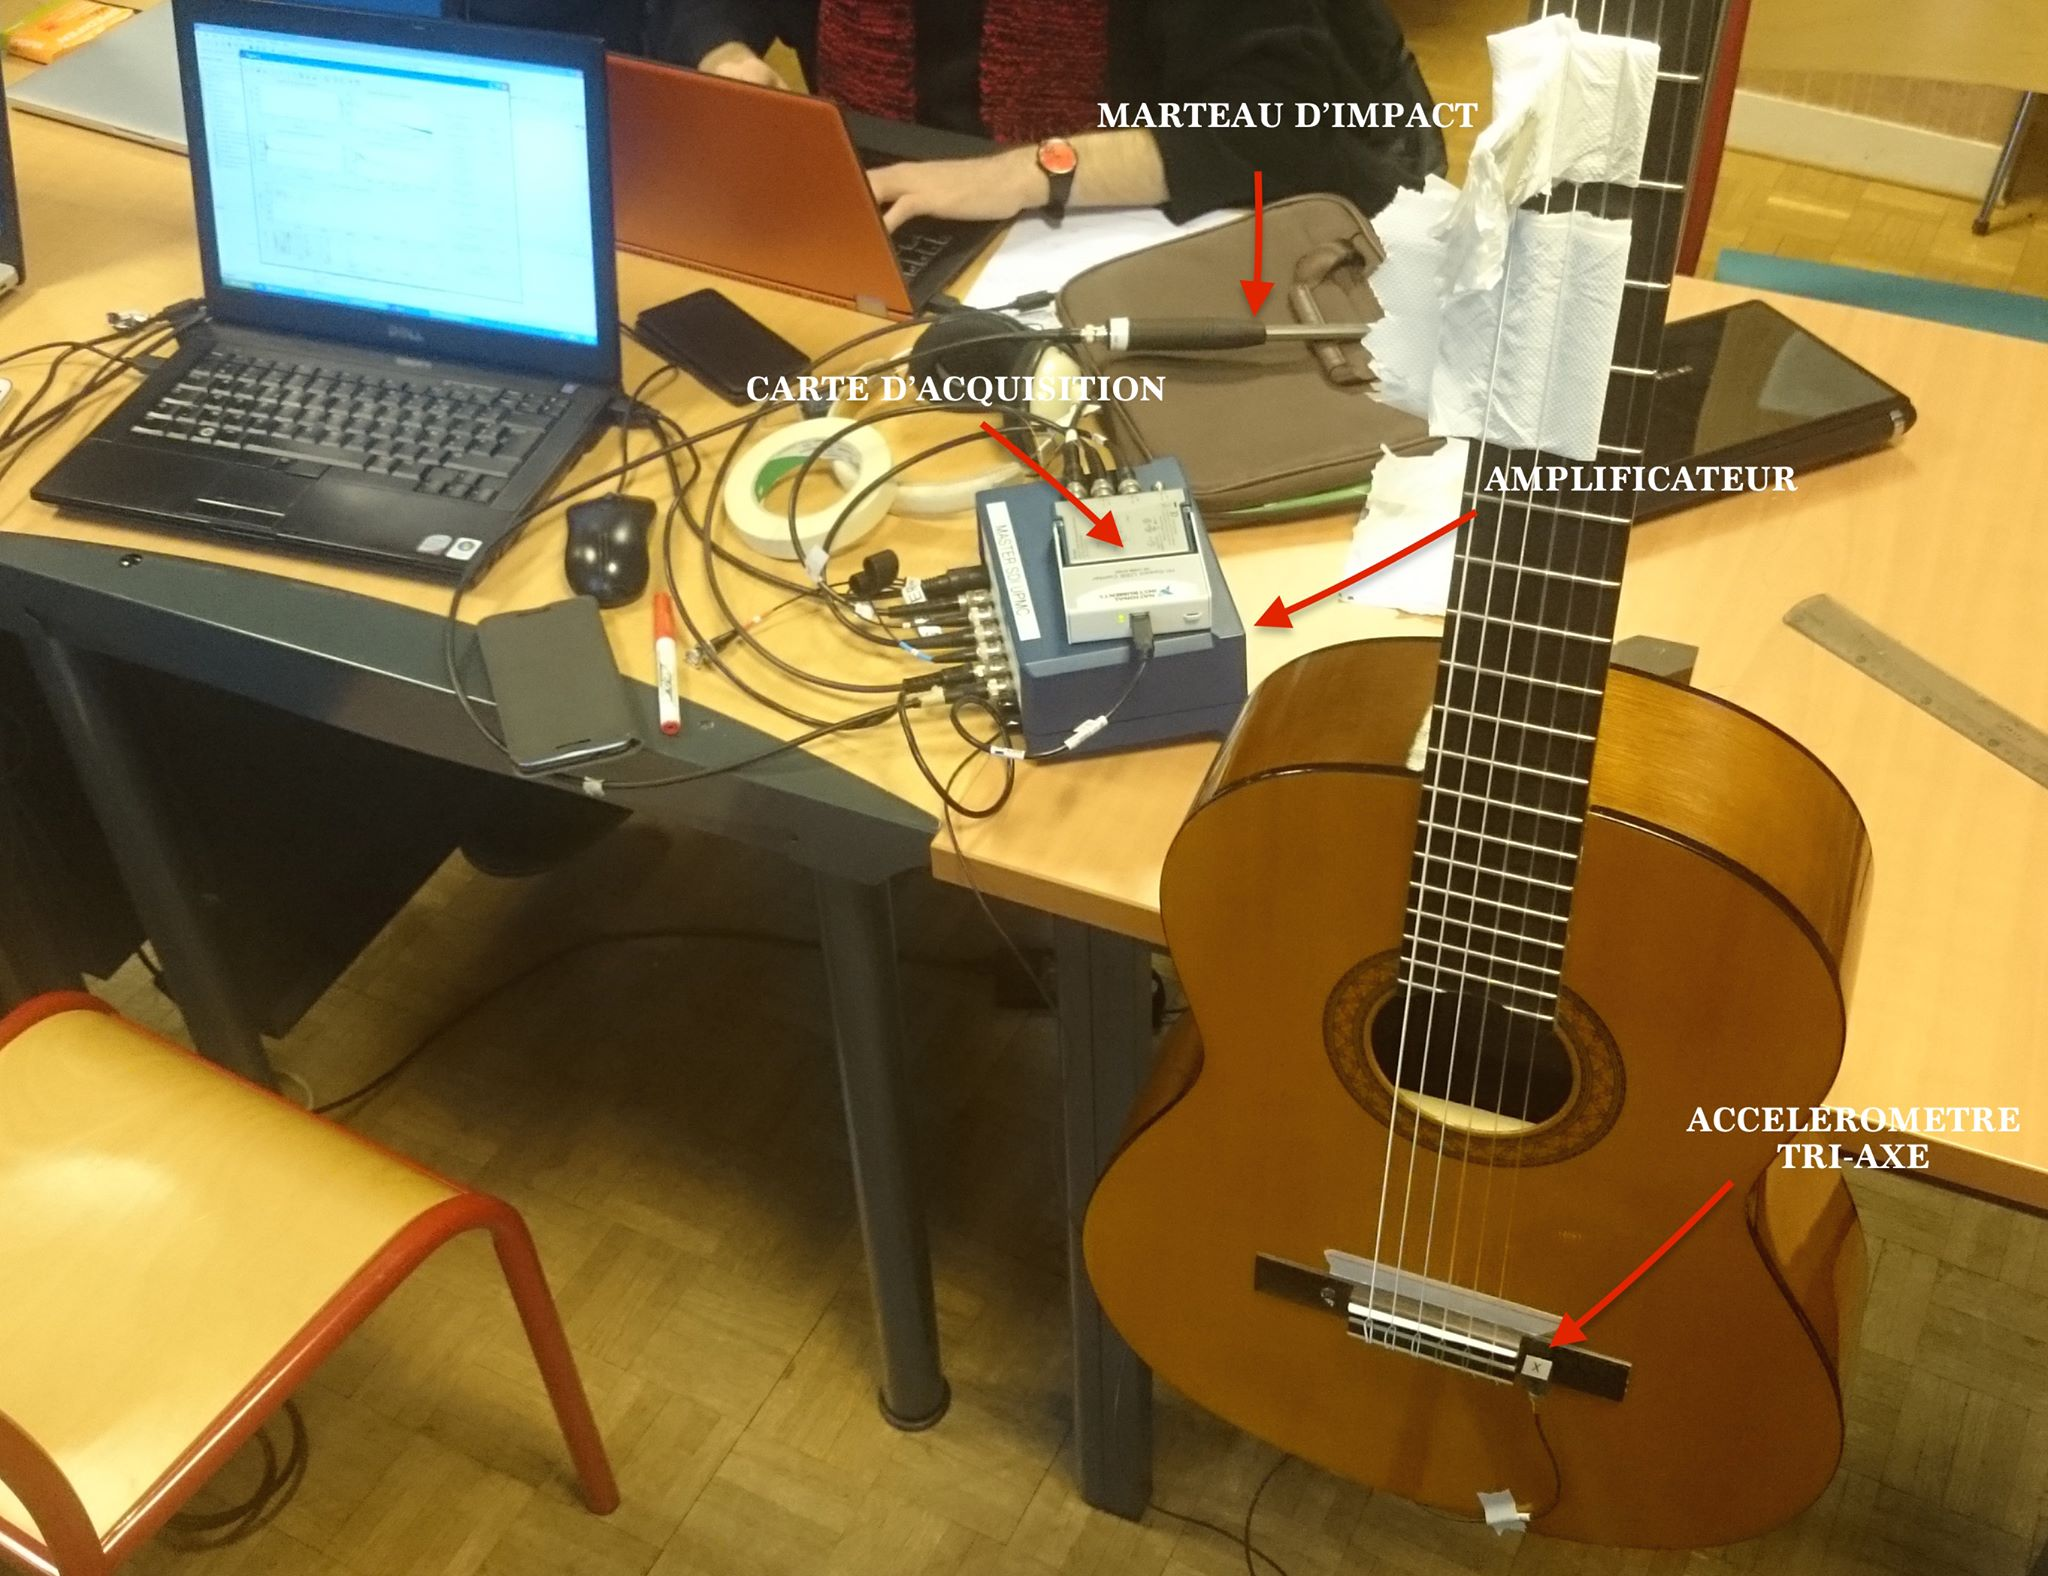
\includegraphics[width = 8cm]{figures/dispo.JPG}
\caption{Dispositif de mesure}
\end{figure}


\subsection{Protocole de mesures}

Voici l'ensemble des mesures effectuées. Pour assurer une répétablité de la
mesure, elles seront faites 5 fois chacune dans le même temps. La  fréquence
d'échantillonnage est fixée à $F_e = 25600Hz$, ce qui nous permet d'obtenir
une bande passante suffisante pour le système à analyser.

\begin{itemize}
\item Mesure à vide pour évaluer le rapport signal sur bruit.
\item Le corps seul, axe vertical(les cordes sont étouffées).
\item Le corps et la corde de Mi2, axe vertical.
\item Le corps et la corde de Mi2, axe horizontal.
\item Le corps et la corde de Mi4, axe vertical.
\item Le corps et la corde de Mi4, axe horizontal. 
\item La corde Mi2 excitée au fil perpendiculairement à la table.
\item La corde Mi2 excitée au fil $45$ degré, à la table.
\item Mesure du rayonnement de la table seule.
\end{itemize}

Pour la première mesure, nous placerons le "target" (force captée au marteau
d'impulsion) proche de zéro dans le but de pouvoir lancer le code d'acquisition
sans impulsion de marteau. \\ Les deux dernières mesures consistent en
l'excitation de la corde à une distance b = 17 mm. 

\subsection{Commentaire et exploitation des résultats}
\subsubsection{Synthèse modale}

Pour la synthèse modale, les modes de corps sont obtenus à partir des mesures
effectués lorsque les cordes étouffées.  L'admittance $Y_{\text{corps}}$ est
ainsi obtenu experimentalement et l'argorithme à haute résolution ESPRIT est
utilisé pour obtenir les fréquences propres et amortissements du système (les
détails de l'approche sont présentés dans la partie ?).  Les modes de corps
sont tantôt obtenus par une estimation haute résolution, tantôt par le modèle
théorique de corde présenté en partie \ref{sec:cordetheo}

\subsubsection{Synthèse fréquentielle}

Pour la synthèse fréquentielle (FRF), les mesures d'$Y_{\text{corps}}$ et
d'$Y_{\text{total}}$ nous permettent d'estimer directement $Y_{\text{total}}$
par une inversion (les détails de l'approche sont présantés dans la partie ?)

\subsubsection{Comparaison et influence de la polarisation}

Les mesures de l'exitation sous plusieurs angles ont pour but d'évaluer
l'influence de la polarisation sur le son produit.  En effet dans le cas d'une
exitation au fil à 45 degrés, l'onde se propage dans la corde selon plusieurs
directions et il est intéressant de comparer si  l'angle d'attaque influence le
son produit.

\subsubsection{Rayonnement acoustique}

Le rapport entre déplacement au niveau du chevalet et la pression rayonnée
permet de determiner une fonction de traduisant du rayonnement acoustique. 
Cette fonction de transfert tient compte des reflections liés aux parois 
de la salle dans lequelle les mesures ont été effectués.

\section{Modèle de corde théorique}
\label{sec:cordetheo}


En parallèle de nos mesures expérimentales, nous construisons un modèle de
corde basé sur les articles de Woodhouse (a) et (b). Le signal temporel de
corde ainsi obtenu sert notament pour vérifier le bon fonctionnement de notre
implémentation de notre algorithme ESPRIT appliquée à un signal temporel de
corde.

Cette synthèse de corde utilise les paramètres suivants : 

\begin{itemize}
\item La raideur ($B$)
\item la masse linéique ($\rho_0$)
\item la tension ($T$)
\item la célérité des ondes ($c_0$)
\item la longueur de la corde ($L$)
\item le point d'excitation ($x_{excitation}$)
\item le point d'écoute ($x_{listening}$)
\item le nombre de modes calculé
\end{itemize}

Ainsi nous pourrons définir l'inharmonicité de la corde comme suit : 
\begin{equation}
w_n = \frac{n\pi}{L} (1+\frac{B}{2T} \frac{n\pi}{L})
\end{equation}

De même, nous avons à notre disposition une façon d'obtenir un amortissement
théorique. Il est soit proposé d'utiliser une valeur constante du facteur de
qualité, \\($Q_{sn} \in [1000 $ $3500]$) soit de le définir à partir des
paramètres de corde : 

\begin{equation}
\eta_{sn} = \frac{T(\eta_F + \eta_A/\omega_n) + B\eta_B(n\pi/L)^2}{T+B(n\pi/L)^2}
\end{equation}
Avec $\eta_F$,$\eta_A$,$\eta_B$ des facteurs de pertes. \\% Ajouter la nature des pertes, je voudrais pas dire de bétises. 

A partir de ces informations, nous pouvons construire l'admittance théorique de la corde, la fonction de transfert force-déplacement, pour la méthode FRF et, construire les matrices solution de l'équation de premier ordre pour la méthode modale.
